\subsection{RBC Modelling Approximation}
\noindent As mentioned in Section \ref{Sect.HS}, this research will focus on spherical \ac{rbc} as starting point. This initial approximation allows the surface stability completed by \citet{Prosperetti1974} and further used by \citet{Zeng2018} to be loosely compared to a \ac{rbc}. However, this comparison between the water droplet and a \ac{rbc} is fundamentally flawed and needs further consideration. 

Figure \ref{fig.rbc.actual} highlights the differences between the water droplet and a \ac{rbc} and identifies the main difficulty in generating a surface stability equation similar to the water droplet material \cite{Prosperetti1974,Zeng2018} for the \ac{rbc}.
\\
\begin{figure}[H]
	\centering
	
	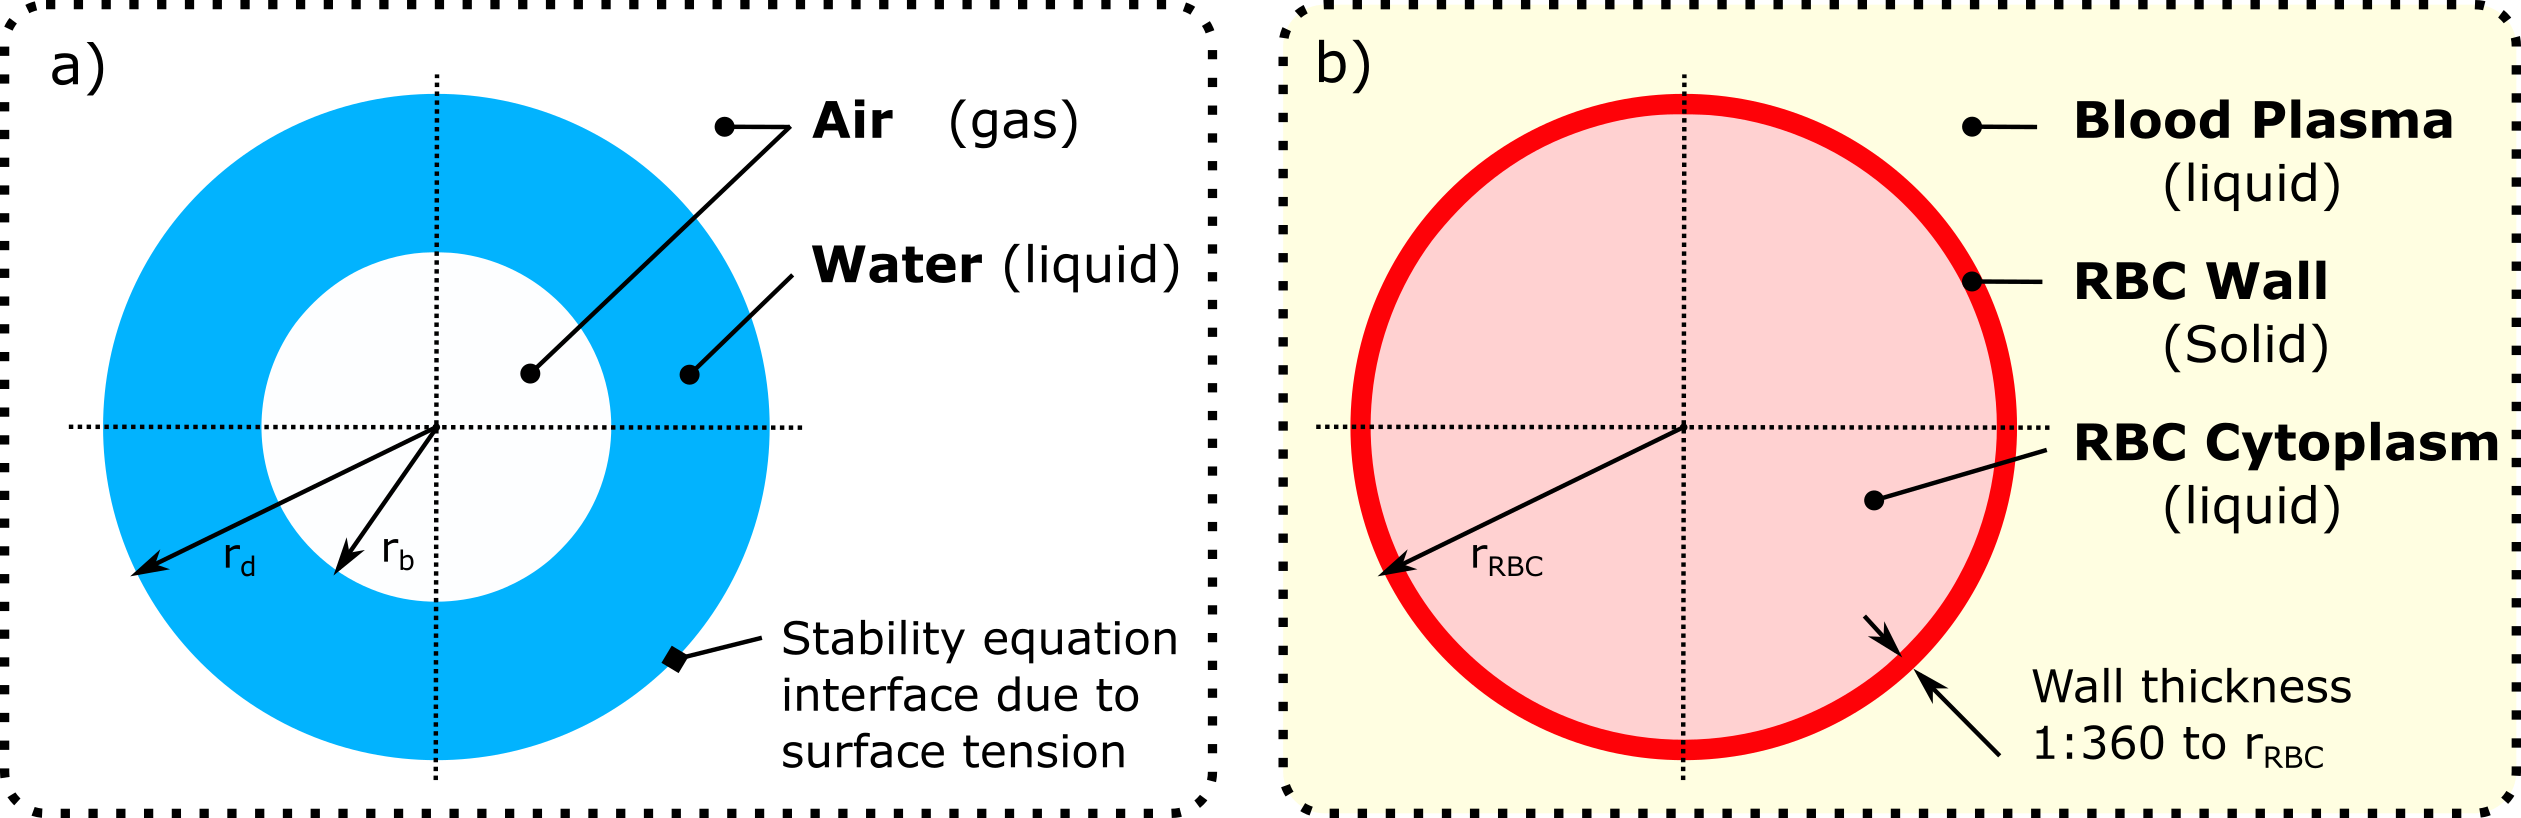
\includegraphics[width=1\linewidth]{fig/Actual}
	
	\caption{Geometry cross-section of a) the water droplet from source material and b) a spherical \ac{rbc}.  }
	\label{fig.rbc.actual}
\end{figure}

\noindent The main difference between the two situations in Figure \ref{fig.rbc.actual} is the occurrence of the solid \ac{rbc} wall. This solid barrier negates the affect of the surface tension between the liquid-gas or liquid-liquid interface. As such changes or simplifications to the \ac{rbc} need to be made to generate a comparable surface stability equation. Figure \ref{fig.rbc.approx} shows three possible approximations of a spherical \ac{rbc} to understand the surface stability. Note, whilst the \ac{rbc} wall is described here as a solid, the cell membrane lipid bilayer is also sometimes referred to a gel-like substance \cite{Himbert2017} who's properties change with temperature. This will be further discussed in Section \ref{Sect.B}. 
\\
\begin{figure}[H]
	\centering
	
	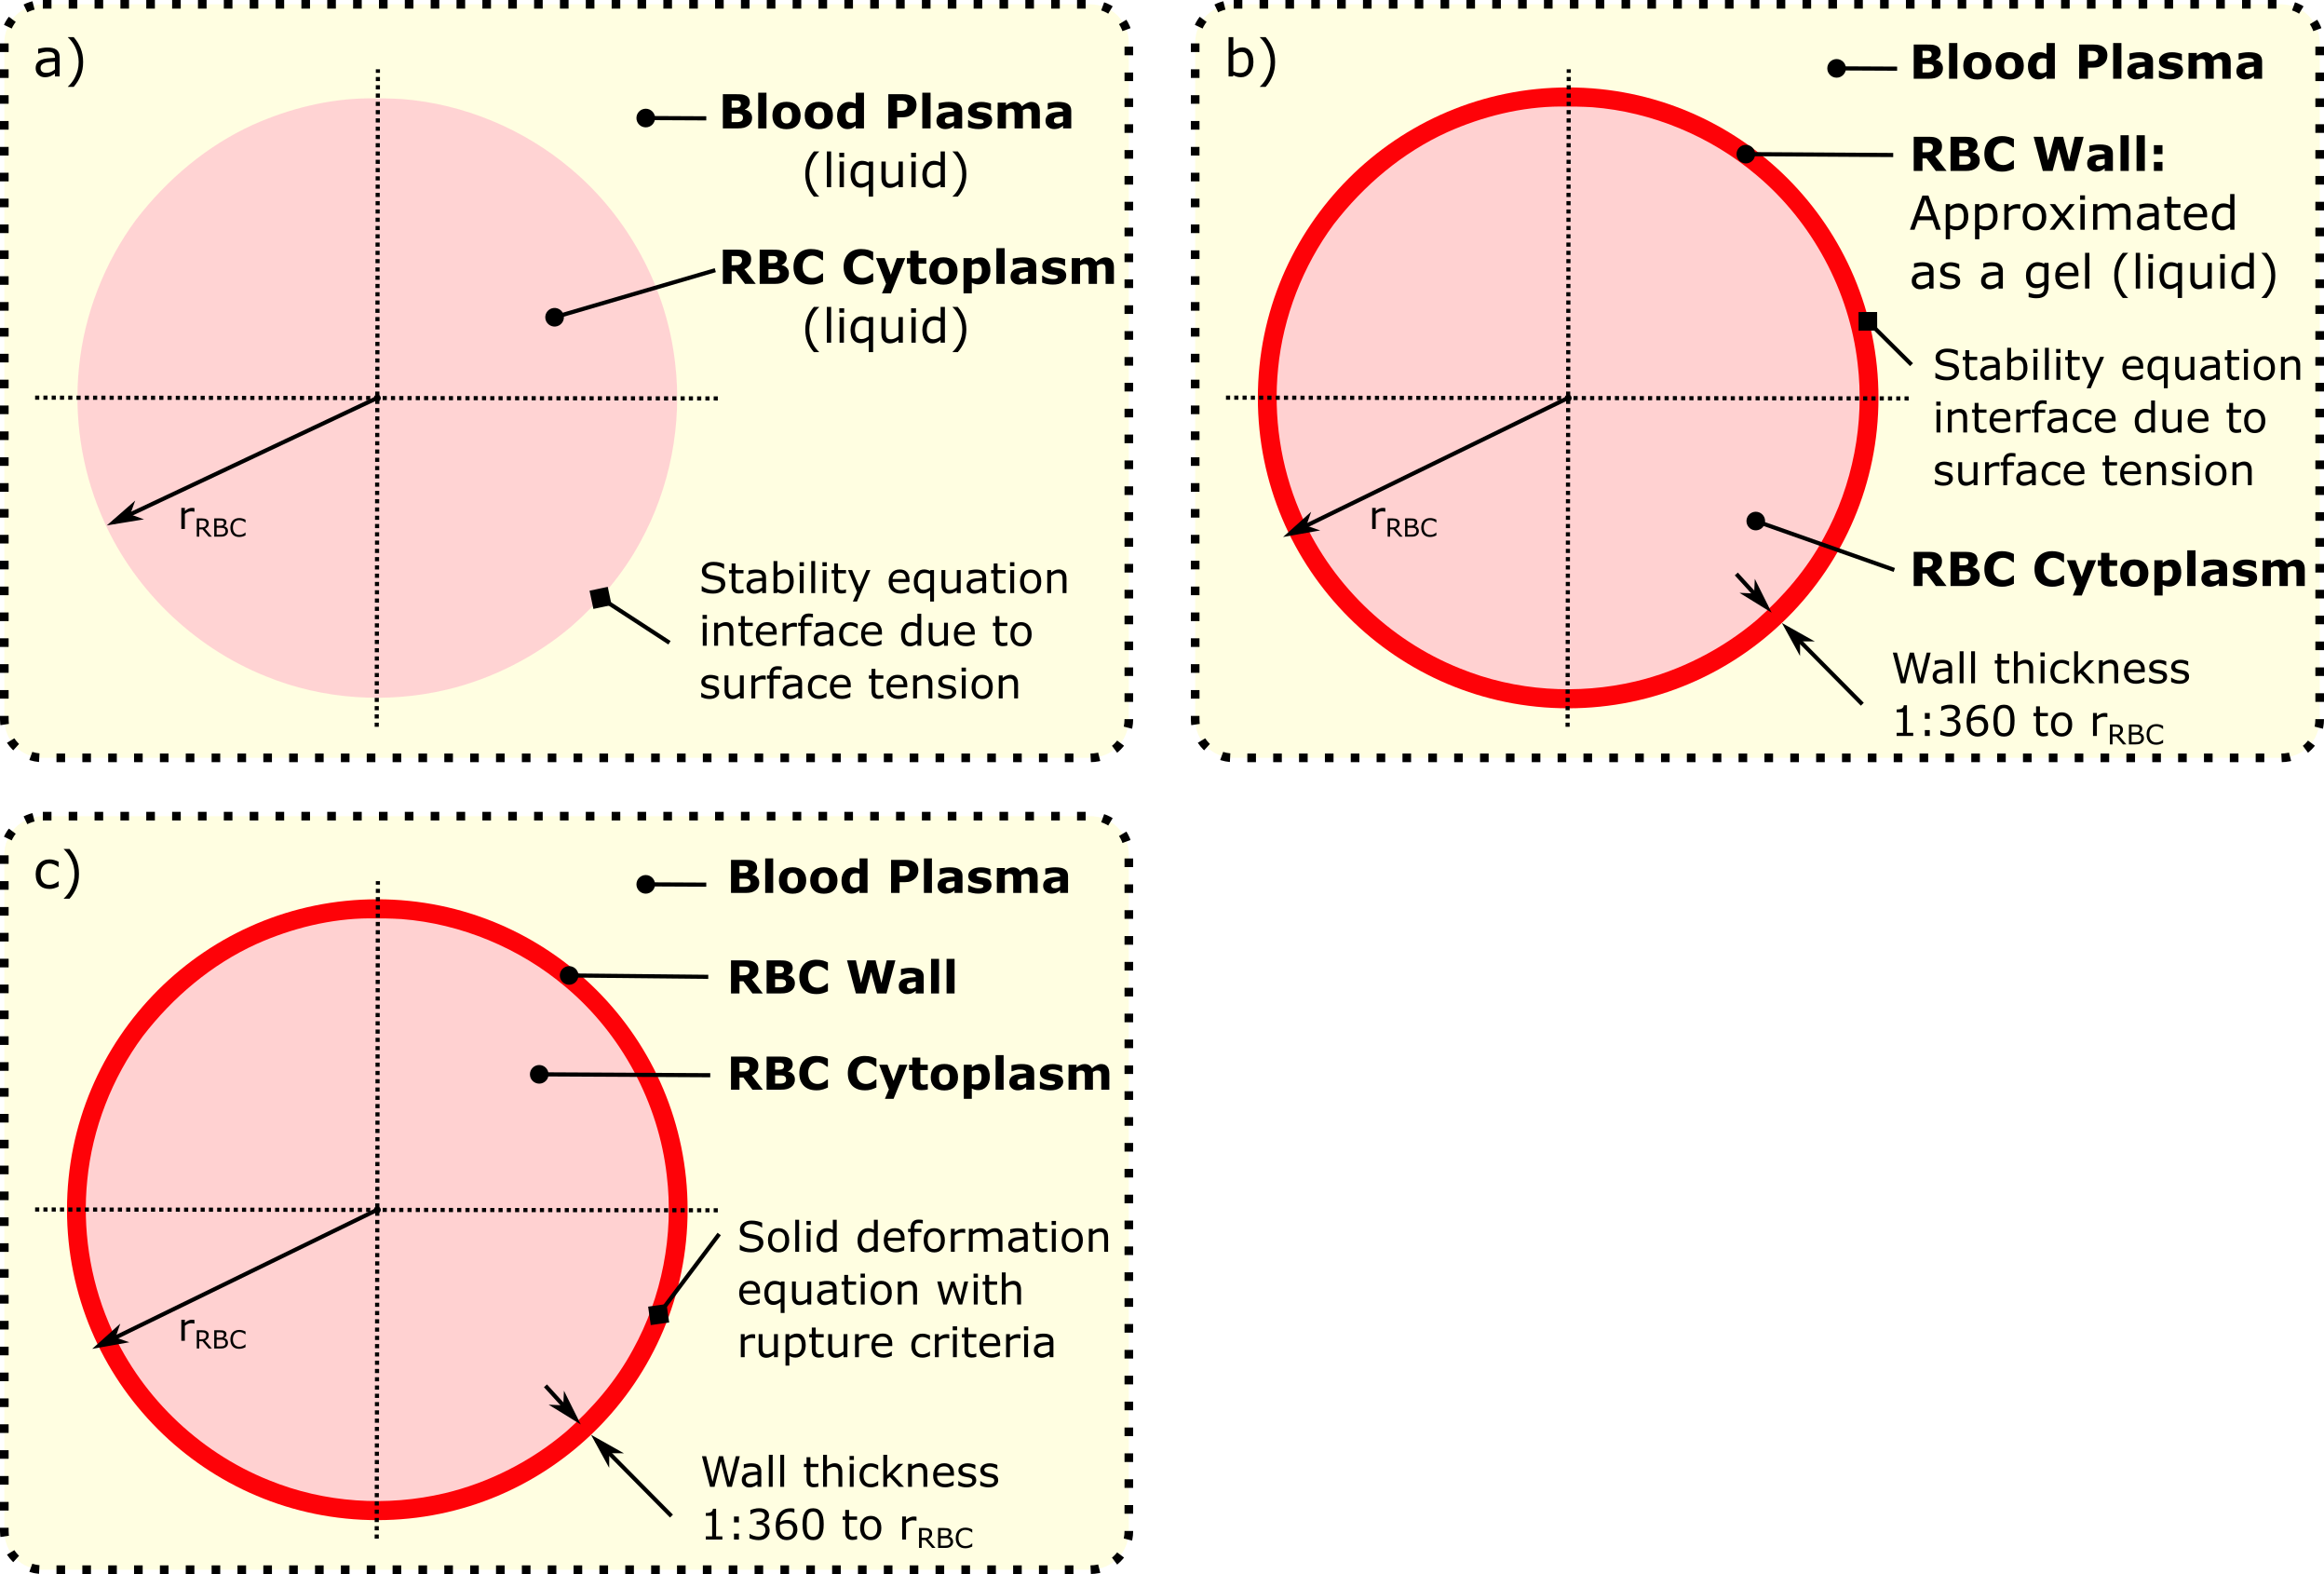
\includegraphics[width=1\linewidth]{fig/approx}
	
	\caption{Possible approximations of the \ac{rbc} in order to generate a surface stability equation. a) makes the assumption that the cell wall is negligible, b) approximates the cell wall as a gel of somewhat comparable properties in order to incorporate the stability equation due to surface tension, and c) substitutes the surface stability equation due to surface tension with a solid deformation equation based upon elastic potential energy.  }
	\label{fig.rbc.approx}
\end{figure}

% How are the two situations differnt
\noindent Each of the three options in Figure \ref{fig.rbc.approx} has associated advantages and disadvantages that need to be considered before implementation. The first of the three options (Figure \ref{fig.rbc.approx}a) assumes that the cell wall can be neglected due to the competitively small thickness when compared to the radius of the cell. This assumption is the least physiological of the three options. However, this assumption allows a direct comparison to the surface stability equation (Equation \ref{eq.der.big}). The second option (Figure \ref{fig.rbc.approx}b) approximates the solid cell wall as a very thin layer of gel liquid instead. The gel approximation allows a similar surface stability equation as \cite{Prosperetti1974,Zeng2018} and option A. For this option it is also assumed that the \ac{rbc} does not rupture as this would result in the model failing. Finally, the third option (Figure \ref{fig.rbc.approx}c) is the most physiological of the three cases, opting to keep the solid cell wall. This option will take a different approach and instead, look at the physical deformation of the cell wall.  However, the disadvantage of the increase in physiological similarity will be increased computation time and mathematical complexity. Again, option C must assume the \ac{rbc} wall does not rupture. 

